% =============================================================================
% Section 1.2 (Part A): Problem Definition
% =============================================================================

\section{Project Objectives and Problem Definition}
\label{sec:problem-objectives}

\subsection{Problem Definition}
\label{subsec:problem-definition}

The central research and engineering problem addressed by this graduation project is stated formally below.

\begin{quote}
\textit{Given a multi-stakeholder e-learning platform serving concurrent students, instructors, and administrators, how can a team design and implement a complete, open, production-ready backend that coordinates authentication, structured course management, video media lifecycles, AI-generated educational content, financial transactions, learner engagement features, and privacy-preserving instructor analytics---while preserving domain clarity across fifteen or more bounded contexts, guaranteeing reliable asynchronous integration with external providers, and maintaining ACID consistency for business-critical state transitions?}
\end{quote}

This overarching problem decomposes into six interrelated sub-problems, each corresponding to observable failure modes in real-world e-learning systems and motivating explicit architectural responses in NexaLearn.

\subsubsection{Lack of Complete Vertical Coverage in Open Backends}
\label{subsubsec:vertical-coverage}

Most publicly available backend templates and partial LMS implementations excel at isolated vertical slices---user registration with JSON Web Tokens (JWT), file upload to object storage, or a basic quiz engine---but fail to implement the \textit{full lifecycle} of a commercial e-learning product within one cohesive domain model. Consider a single paid enrollment: the system must validate course availability and pricing, create a pending enrollment record, initiate a Stripe PaymentIntent, await a signed webhook confirming payment, atomically activate enrollment, initialise progress projections for all lessons, grant Mux playback entitlements, enqueue welcome notifications, update search-facing enrollment statistics, and record audit events---all while remaining resilient to duplicate client retries and partial failures.

When these concerns are implemented as an undifferentiated ``services'' layer without bounded contexts, implicit coupling emerges rapidly. Payment services begin mutating enrollment tables directly; progress services bypass assessment prerequisites; search reads denormalised columns that drift when outbox processors lag. The sub-problem is therefore not merely absent features, but the absence of a \textit{ubiquitous language} and \textit{context map} assigning ownership, invariants, and published integration contracts to each concern. NexaLearn responds by defining sixteen domain modules---Auth, Courses, Enrollment, Payments, Media, AI Pipeline, Assessment, Discussion, Progress, Reviews, Certificates, Search, Streak, Notifications, Instructor, and Admin---plus infrastructure modules for Prisma, Events, and Audit.

\subsubsection{Unreliable Asynchronous Event Processing}
\label{subsubsec:async-events}

E-learning backends are inherently event-heavy. Representative external event sources include:
\begin{itemize}
  \item \textbf{Mux webhooks} --- \texttt{video.asset.ready}, upload cancellation, encoding errors;
  \item \textbf{Stripe webhooks} --- \texttt{payment\_intent.succeeded}, \texttt{payment\_intent.payment\_failed}, \texttt{charge.refunded}, \texttt{checkout.session.completed};
  \item \textbf{AI pipeline callbacks} --- transcription completion, generated question payloads, grading results for short-answer items;
  \item \textbf{Internal domain events} --- \texttt{EnrollmentActivated}, \texttt{LessonCompleted}, \texttt{QuizAttemptSubmitted}, \texttt{CertificateIssued}.
\end{itemize}

Network partitions, at-least-once delivery guarantees from cloud providers, and application restarts during consumer processing make duplicate and out-of-order delivery \textit{normal} rather than exceptional. Naive ``publish to message broker after commit'' approaches suffer the dual-write problem: database commits succeed while message publication fails, or vice versa. NexaLearn must achieve \textit{at-least-once transport with exactly-once side effects} without two-phase commit across heterogeneous systems. The chosen pattern---\textbf{transactional outbox} with row-level locking via \texttt{SELECT FOR UPDATE SKIP LOCKED}---persists events in the same PostgreSQL transaction as domain mutations, then processes them idempotently through dedicated handlers that update projections, dispatch notifications, and trigger downstream workflows.

\subsubsection{Architectural Erosion Across Many Bounded Contexts}
\label{subsubsec:bounded-context-erosion}

Domain-Driven Design recommends decomposing complex domains into bounded contexts with explicit upstream/downstream relationships, anti-corruption layers for external models, and context maps documenting integration styles (shared kernel, customer-supplier, conformist, open-host service). In practice, naively creating fifteen or more NestJS modules without enforced dependency rules yields circular imports, anaemic entities that mirror database rows without behaviour, and repository leakage where controllers query foreign context tables directly.

The sub-problem is organisational and technical: maintain Clean Architecture layering (domain innermost; application use cases; infrastructure adapters outermost) across twenty NestJS modules while preserving developer velocity. Dependency constraints require that Courses never import Payments repositories; Discussion never writes Progress tables; Instructor analytics reads through authorised query services rather than ad hoc joins. Without discipline, the modular monolith collapses into the monolithic ``ball of mud'' it was intended to prevent.

\subsubsection{Exactly-Once Semantics for Financial and AI Integrations}
\label{subsubsec:financial-ai-integrity}

Monetary transactions and machine-generated assessments carry elevated correctness, regulatory, and reputational requirements. Failure modes include:
\begin{itemize}
  \item duplicate Stripe webhook $\rightarrow$ double enrollment activation or duplicate revenue recognition;
  \item lost refund webhook $\rightarrow$ student retains access after chargeback;
  \item replayed AI callback $\rightarrow$ duplicate quiz questions or overwritten instructor edits;
  \item forged unsigned callback $\rightarrow$ injection of malicious assessment content.
\end{itemize}

Conversely, legitimately retried webhooks after transient 503 responses must succeed without manual operations intervention. NexaLearn must implement \textit{idempotent, auditable integration endpoints} with Stripe signature verification, HMAC-authenticated AI pipeline callbacks, structured correlation identifiers (\texttt{enrollmentId}, \texttt{pipelineJobId}, \texttt{idempotencyKey}), and persistent deduplication stores recording processed event fingerprints.

\subsubsection{Privacy-Preserving Instructor Analytics}
\label{subsubsec:privacy-analytics}

Instructors require aggregated insights---module completion funnels, median quiz scores, revenue by course offering, streak participation rates, discussion engagement---to improve content and pricing decisions. Platform administrators require security dashboards (failed login spikes, token reuse alerts). However, indiscriminate SQL joins across \texttt{User}, \texttt{Enrollment}, \texttt{LessonProgress}, and \texttt{Payment} tables risk exposing personally identifiable information (PII), enabling re-identification in small cohorts, or allowing Instructor~A to infer performance data for courses they do not own.

The sub-problem is to deliver \textit{actionable analytics through dedicated application services} that enforce role-based access control (RBAC), aggregate at safe granularities, parameterise queries by \texttt{instructorId} derived from authenticated identity rather than client-supplied filters, and never return row-level student identifiers in instructor-facing revenue or engagement exports unless explicitly authorised for institutional admin roles.

\subsubsection{Stakeholder Expectations and Non-Functional Constraints}
\label{subsubsec:stakeholder-nfr}

Beyond functional gaps, the problem includes satisfying diverse stakeholder non-functional requirements simultaneously. Table~\ref{tab:stakeholder-requirements} maps primary stakeholders to expectations that constrain architecture.

\begin{table}[H]
  \centering
  \caption{Stakeholder Groups and Their Architectural Expectations in NexaLearn}
  \label{tab:stakeholder-requirements}
  \small
  \begin{tabular}{@{}p{2.6cm} p{4.2cm} p{6.8cm}@{}}
    \toprule
    \textbf{Stakeholder} & \textbf{Primary Concerns} & \textbf{Architectural Implications} \\
    \midrule
    Students &
    Fair access after payment; reliable video playback; accurate grades &
    Idempotent enrollment activation; signed Mux URLs; atomic quiz finalisation \\
    \addlinespace
    Instructors &
    Content control; AI assistance; performance insights &
    OCC on course aggregates; AI job tracking; scoped analytics queries \\
    \addlinespace
    Platform admins &
    Security; auditability; moderation &
    RBAC; Audit module; admin dashboards; rate limiting \\
    \addlinespace
    Developers &
    Maintainability; testability; clear boundaries &
    DDD modules; outbox tests; OpenAPI docs; Docker Compose \\
    \addlinespace
    Evaluators &
    Reproducibility; self-contained documentation &
    Migrations; integration tests; this report \\
    \bottomrule
  \end{tabular}
\end{table}

\begin{figure}[H]
  \centering
  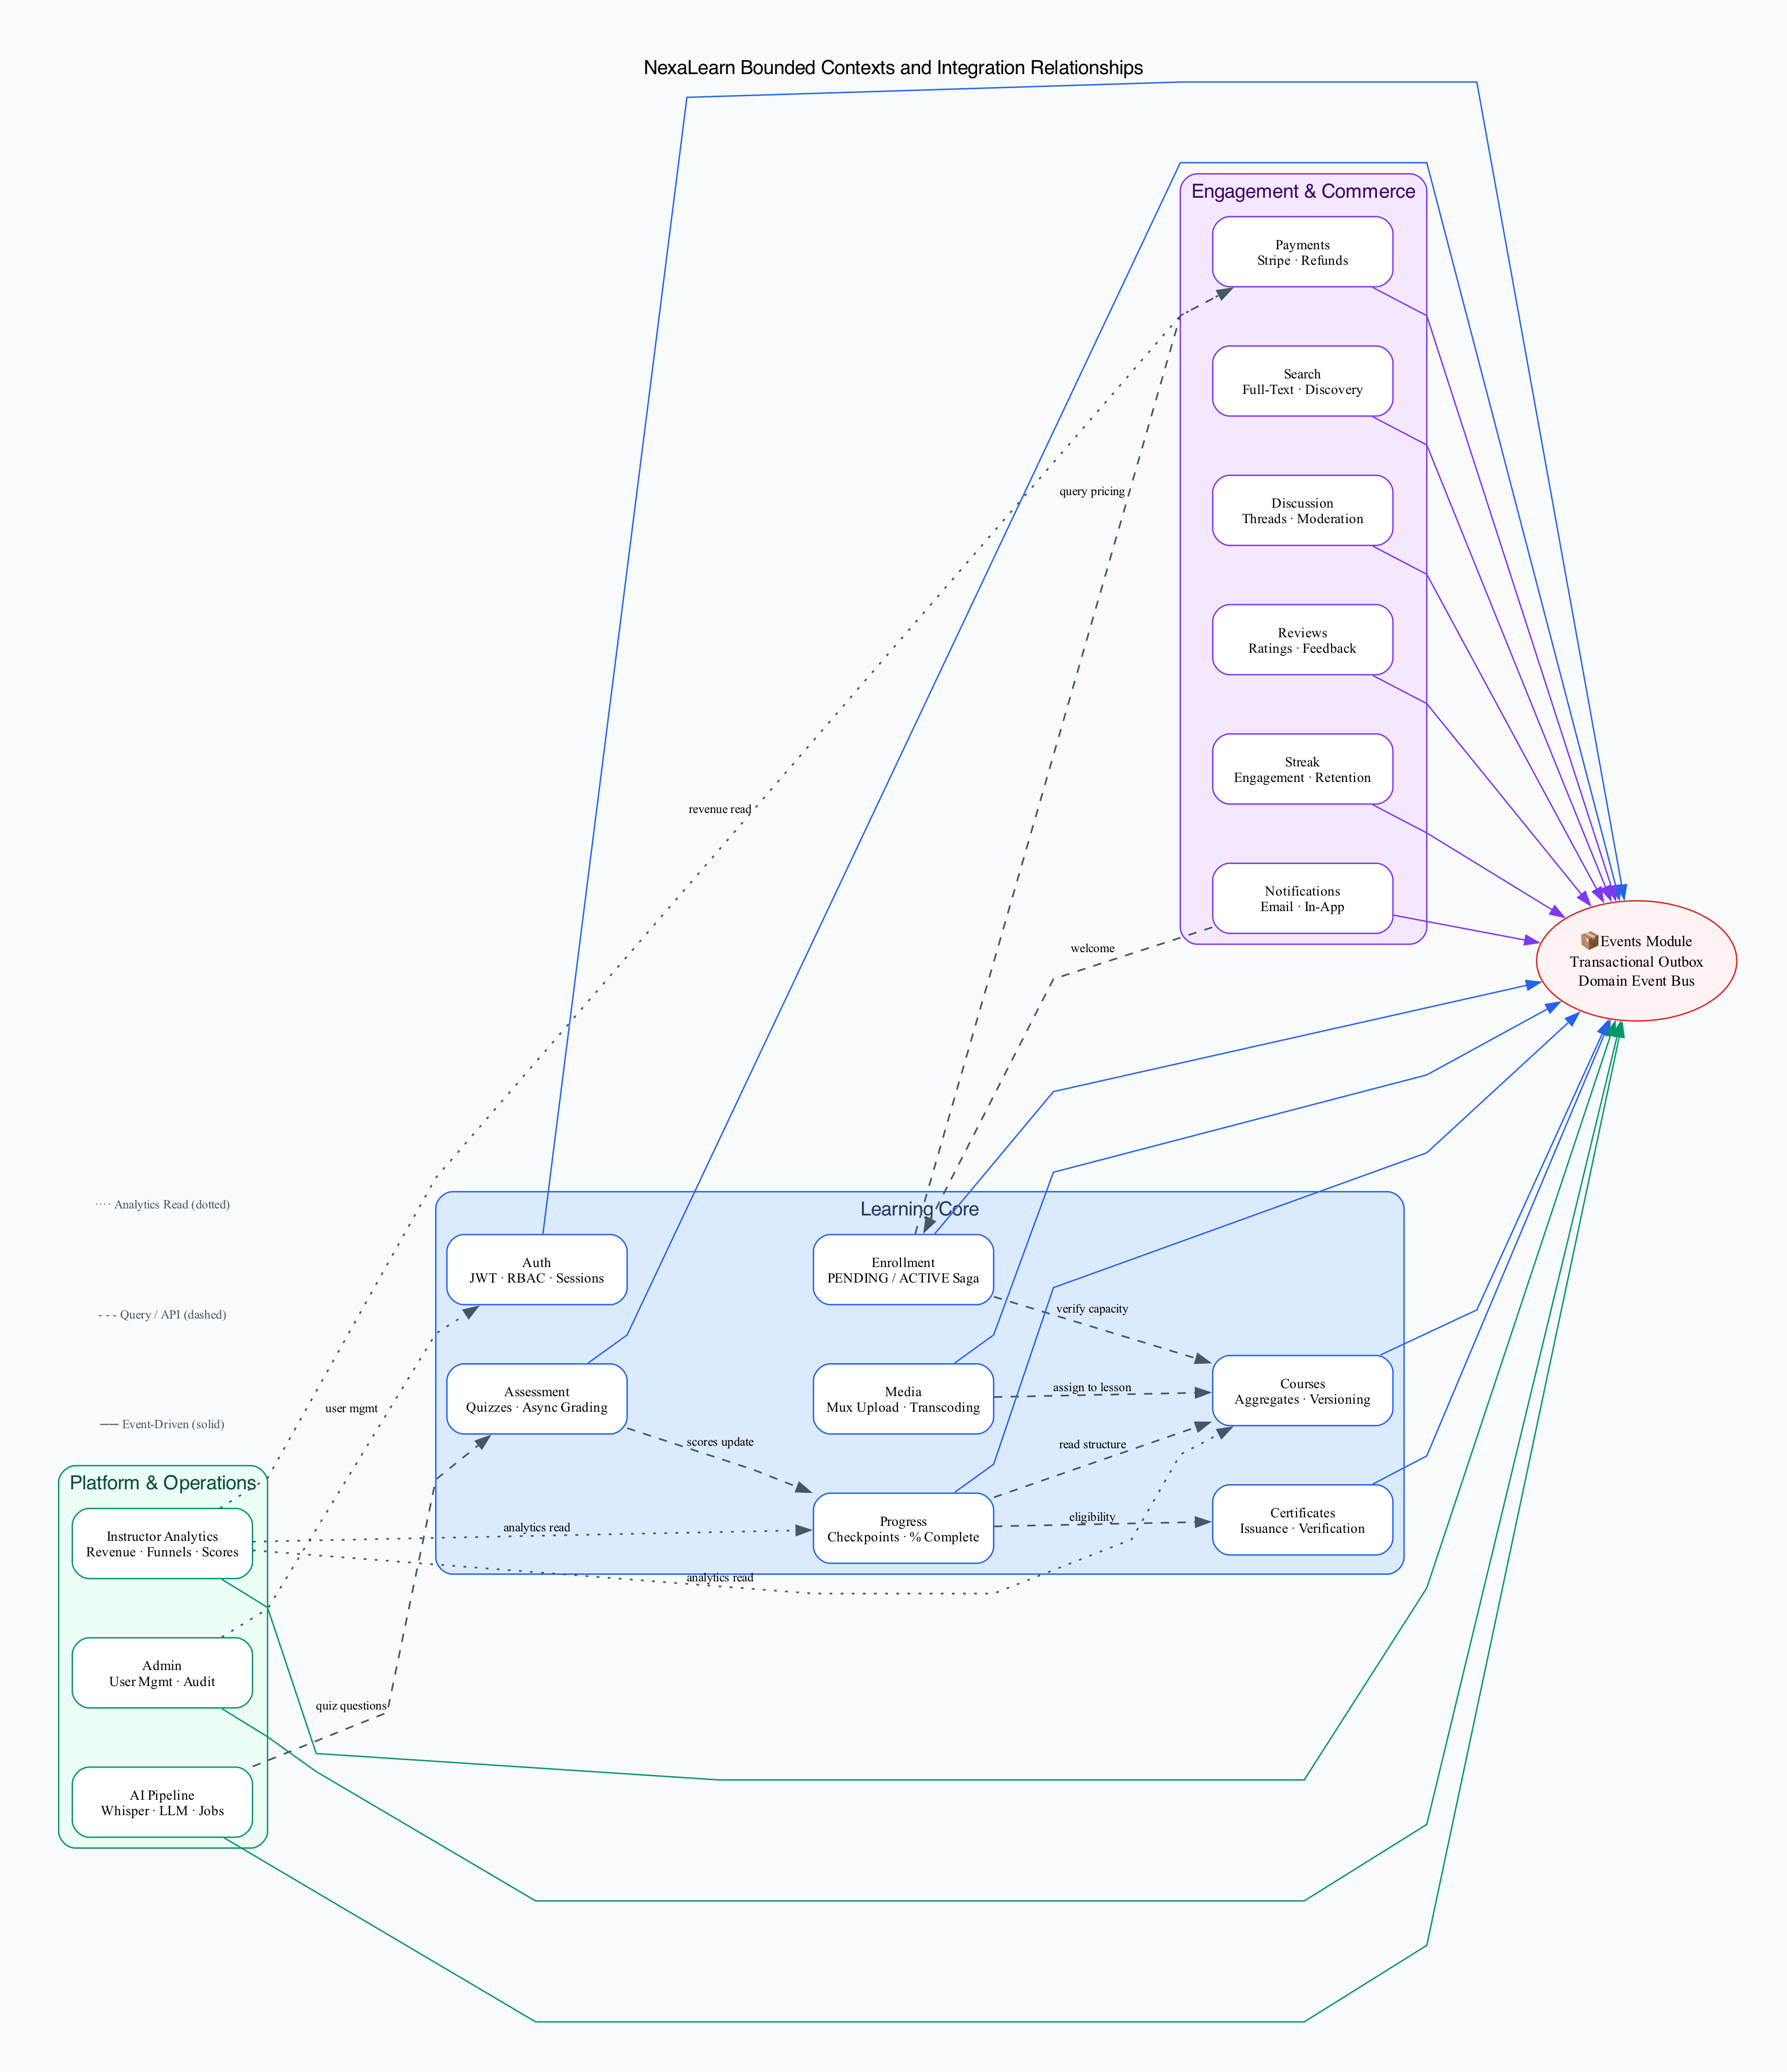
\includegraphics[width=0.88\textwidth]{images/bounded_contexts.png}
  \caption{NexaLearn Bounded Contexts and Integration Relationships}
  \label{fig:bounded-contexts}
\end{figure}

Figure~\ref{fig:bounded-contexts} visualises the sixteen domain bounded contexts and their primary event-driven (solid) and query/API-driven (dashed) relationships. Three high-level groupings---Learning Core, Engagement \& Commerce, Platform \& Operations---provide cognitive structure without implying separate deployable microservices. The Events module and transactional outbox sit centrally because nearly every context publishes or consumes domain integration events.

Collectively, these sub-problems define a problem space where superficial feature accumulation fails; only explicit domain modelling, reliability patterns, and layered architecture can produce a backend that remains correct under concurrency, trustworthy under duplicate webhooks, and comprehensible to engineers who inherit the codebase after graduation.
